\documentclass[acmsmall,screen]{acmart}
\setcopyright{none}
\copyrightyear{2022}
\acmYear{2022}
\acmDOI{}

\citestyle{acmauthoryear}

\usepackage{fancyhdr}
\usepackage{float}
\usepackage{listings}
\usepackage{caption}
\DeclareCaptionFont{white}{\color{white}}
\DeclareCaptionFormat{listing}{%
  \parbox{\textwidth}{\colorbox{gray}{\parbox{\textwidth}{#1#2#3}}\vskip-4pt}}
\captionsetup[lstlisting]{format=listing,labelfont=white,textfont=white}
\lstset{frame=lrb,xleftmargin=\fboxsep,xrightmargin=-\fboxsep}

\begin{document}

\title{Animato: A Domain-Specific Language for Animation and Drawing}

\author{Daniel Son}
\email{danielson@college.harvard.edu}
\affiliation{%
  \institution{Harvard University}
  \country{USA}
}

\renewcommand{\shortauthors}{Daniel Son}

\settopmatter{printacmref=false}
\settopmatter{printfolios=true}
\renewcommand\footnotetextcopyrightpermission[1]{}
\pagestyle{fancy}
\fancyfoot{}
\fancyfoot[R]{CS252R (Fall 2024)}
\fancypagestyle{firstfancy}{
  \fancyhead{}
  \fancyhead[R]{CS252R (Fall 2024)}
  \fancyfoot{}
}
\makeatletter
\let\@authorsaddresses\@empty
\makeatother

\begin{abstract}
    Animato is a domain-specific language aimed to tackle the problem of tedious drawing for animation and shape rendering.
    While there exists tools such as p5.js~\cite{p5js} and Penrose~\cite{penrose}, this project mimics and extends certain aspects of existing tools.
    We design a domain-specific language that takes shape inputs with locations and outputs the drawings on a canvas as a \texttt{.png} file.
    Depending on the input, the output may be a singular or multiple image files where the sequence of image files can be input into an animation software such as Adobe Premiere Pro or TV Paint to create an animation.
\end{abstract}

% \keywords{music synthesis, first species counterpoint, domain specific language, programming languages}

\maketitle
\thispagestyle{firstfancy}

\section{Introduction}
Art is prevalent in all shapes and forms, one being visual.
In the field of animation, drawing is a tedious yet important task that 2-dimensional animators often have to utilize.
Due to the tedious nature of hand-drawn animation, Animato aims to relieve animators of the need to draw each frame and develop animations using the domain-specific language.

\subsection{Related Work}
Previously, much work has been done in the p5.js \cite{p5js} community as well as the Penrose \cite{penrose} CMU community to advance the code in art space. 
p5.js is an open-source JavaScript library that aims to make creative coding accessible to artists and coders alike. 
Similarly, Penrose provides a tool to allow users to create complex diagrams that would otherwise be hard to depict in a formal setting.

\begin{center}
  \begin{figure}[!h]
    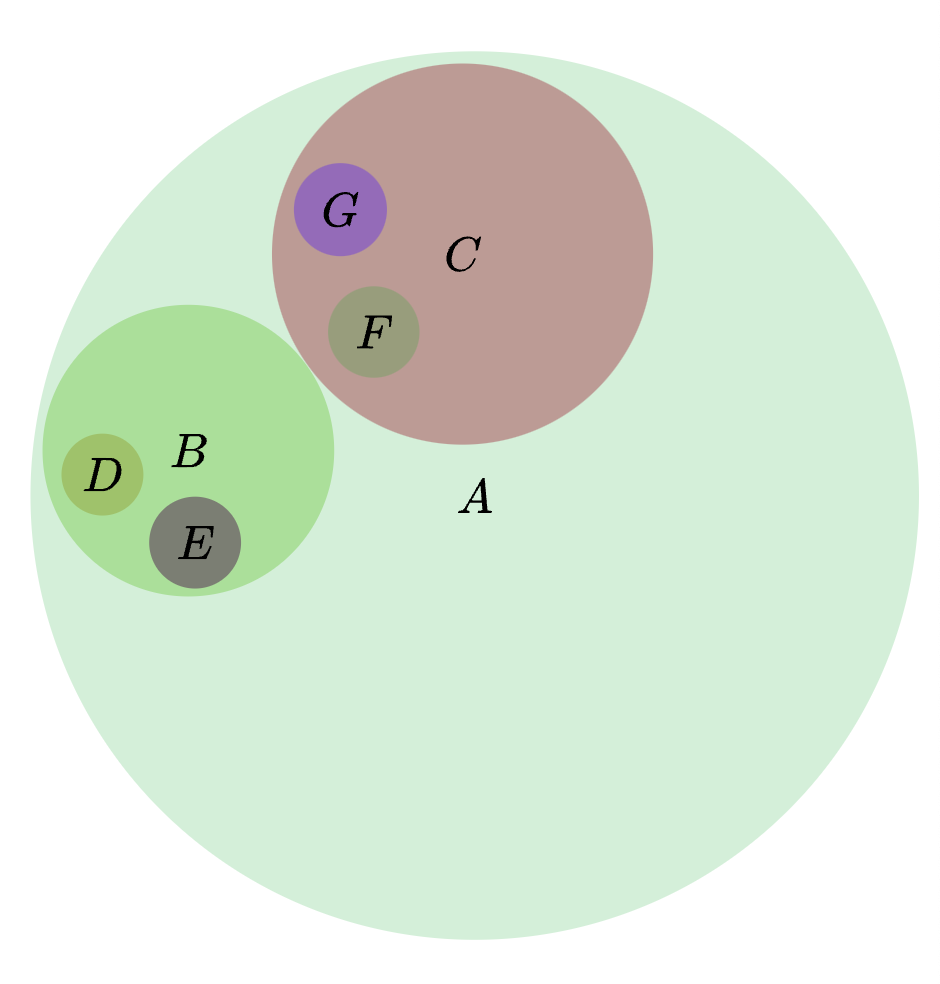
\includegraphics[width=0.49\textwidth]{images/penrose.png}
    \caption{Example diagram created in Penrose of sets}
  \end{figure}
\end{center}

\noindent The overall goal of these languages and libraries is to provide an easier and more precise way to create drawings.
In this project, we attempt to recreate features of p5.js and Penrose in Animato's language and extend certain functionality to be more specialized.
While Animato is not necessarily novel, it aims to be a more general and user-friendly langauge for animators who do not need to understand the backend.

\section{Framework}
\subsection{Primitives}
In the current iteration of Animato, there are multiple primitives for shapes that are ready to be utilized.
These include squares, circles, line segments, and some other harder to achieve common shapes. 
While circles and squares are predefined shapes, lines can be drawn and connected with other lines to create more complex shapes.
In the future, it would be very beneficial to implement a primitive to create bezier curves.
The addition of bezier curves would allow users to create shapes that are less rigid (e.g. a cloud shape).

\begin{center}
  \begin{figure}[!h]
    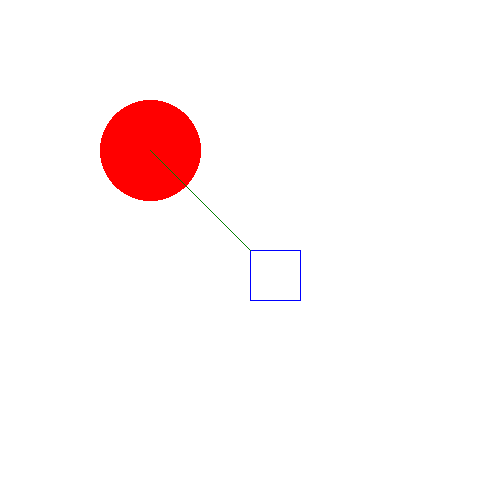
\includegraphics[width=0.49\textwidth]{images/primitives.png}
    \caption{Example of circle, square, line segment primitives on canvas}
  \end{figure}
\end{center}

\subsection{Implementation}
Animato uses a Python backend with Pillow for drawing visualizations, z3 for constraint solving, and PLY/sexpr for parsing and intepretting the input.
At the current state, running the \texttt{main.py} file with a valid \texttt{dsl\_code} input will only produce one file.
The file is a visual representation of the input given with precise locations and relationships.

\section{Example}
Using these primitives, users are able to create custom shapes (functions) by defining a function as follows:

\begin{lstlisting}[label=code, caption=Sample custom function definition in Animato]
    dsl_code = """
      (define star (cx 0) (cy 0) (radius 50) (
        (line (x1 (- cx radius))
              (y1 (- cy radius))
              (x2 (+ cx radius))
              (y2 (+ cy radius)))
        (line (x1 (- cx radius))
              (y1 (+ cy radius))
              (x2 (+ cx radius))
              (y2 (- cy radius)))
        (line (x1 cx) (y1 (- cy radius))
              (x2 cx) (y2 (+ cy radius)))
        (line (x1 (- cx radius)) (y1 cy)
              (x2 (+ cx radius)) (y2 cy))
      ))
      (star (cx 250) (cy 250) (radius 100))
    """
\end{lstlisting}

\begin{center}
  \begin{figure}[!h]
    
\includegraphics[width=0.5\textwidth]{images/star.png}
    \caption{Output image of \texttt{dsl\_code} input for a star}
  \end{figure}
\end{center}

The above \texttt{dsl\_code} input produces the drawing shown in figure 1.

\section{Limitations and Future Work}
While the intent of this project is to create a domain-specific language to assist programmers and animators to easily draw animations, there is still work that needs to be done in order to flesh out this idea.
Firstly, the aspect of custom-defined functions is quite limited and Animato needs more functionality that gives a more user-friendly experience.
While the aim of Animato is to allow everyone to create animations without the need to look in the backend to see what it's doing, this is quite difficult to allow users to actually do whatever they want.
In testing, it has been apparent that actually creating custom functions is quite hard since the user needs a precise understanding of the canvas space.
Further, without bezier curves, users are not able to create curved shapes making the scope of possible shapes limited.
In future iterations of Animato, the main focus should be to create a more user-friendly experience and more functionality in the language itself.
While not in the scope for this project, ideally users would be able to create a shape in the \texttt{dsl\_code} input and have a live view of the canvas.
Currently, the only way to test the drawings is by running \texttt{main.py} and checking the \texttt{output.png} file. 

\section{Conclusion}
Overall, while the aim of Animato is to provide a more concise and specialized language for animators/developers to use, further work must be done to polish the domain-specific langauge.
At the current state, users are able to create a canvas with some specified shape drawings, including custom shapes.
Further work should be done to extend the usability and enhance existing features.
This project acts as a foundation that can be extended for more utility.

\begin{acks}
This paper and project serves as my final project for CS 252, Advanced Programming Languages, at Harvard University. Special thanks to Professor Nada Amin, Raffi Sanna, and classmates in CS 252 for providing feedback and advice on the project in it's developmental stage.
\end{acks}

\bibliography{references}
\bibliographystyle{ACM-Reference-Format}

\end{document}